% !TeX program = pdflatex
% !TeX encoding = UTF-8
\documentclass[runningheads,a4paper]{llncs}
\usepackage[T1]{fontenc}
\usepackage{amsmath,amssymb,graphicx}
\usepackage{multirow}
\usepackage{float}
\usepackage{subcaption}
\renewcommand{\labelitemi}{\textbullet}
% Permit a little extra interword stretch only when normal line breaking fails.
\setlength{\emergencystretch}{2em}
% Visible drafting markers; remove each one only after its evidence is supplied.
\title{Cross-City Transfer Learning for Traffic Forecasting with Limited Training Data}
\titlerunning{Cross-City Transfer Learning for Traffic Forecasting}
\author{Anonymous Authors}
\authorrunning{Anonymous Authors}
\institute{}
\begin{document}
\maketitle

\begin{abstract}

Traffic forecasting supports transportation management and urban planning.
In real-world traffic forecasting applications,  nodes may lack historical traffic observations during training.
Existing approaches leverage local data augmentation to generate extra training sequences, yet they still depend on temporal patterns captured from the limited nodes with available training data.
Driven by this limitation, we propose \emph{CrossGEN}, short for Cross-city Generator transfer, which augments local patterns with knowledge learned from a source city for traffic forecasting.
CrossGEN uses a window generator to synthesize training sequences, a graph generator that constructs the target graph from node histories, and a spatiotemporal graph neural network backbone to forecast traffic.
To transfer these source-pretrained modules to the target city with only a small set of nodes with training observations, CrossGEN further adopts a target adaptation pipeline that regularizes transferred parameters toward their source values.
We evaluate CrossGEN on five traffic flow datasets and two traffic index datasets with 10\% of target nodes with training data. Experiments show that CrossGEN significantly outperforms the baselines in most cases, demonstrating the effectiveness of our method.


\keywords{Traffic forecasting \and cross-city transfer learning \and spatiotemporal graphs \and virtual nodes \and inductive forecasting.}
\end{abstract}

\section{Introduction}
Traffic  forecasting supports real-time decisions in urban road networks.

However, in real-world traffic forecasting applications, most nodes may lack historical traffic observations during training. For instance, a city may build new roads after training its model, adding nodes to the road network. When the new roads open and recent observations become available, operators need traffic forecasting for the new nodes.
\iffalse Traffic demand follows daily and weekly cycles, and congestion spreads across neighboring roads. Since spatial-temporal graphs record both the spatial relations among nodes and each node's temporal evolution, spatial-temporal graph neural networks (STGNNs)~\cite{stgcn,graphwavenet} are widely used for this task. However, such models still require temporal data at every node. The temporal pattern of a node is learned from its own data, so a node that provides no temporal data is forecast poorly. \fi
ST-FiT~\cite{stfit} generates synthetic time series for training by mixing latent representations of the available histories.
However, temporal patterns that rarely occur at the observed nodes may remain underrepresented after augmentation.

Cross-city transfer uses historical traffic observations from one or more cities to improve traffic forecasting in another city (i.e., the target city).
ST-GFSL~\cite{stgfsl} transfers node-level knowledge, and TransGTR~\cite{transgtr} transfers a graph generator and a forecaster.
Both studies adapt their models using short histories from all nodes in the target city, leaving open whether transfer helps when only a small subset supplies training data.
For example, after a city expands sensor coverage, all monitored nodes can provide recent observations at inference even though only the original nodes supplied training data.
We therefore investigate whether source-city pretraining improves traffic forecasting at target nodes with no training history.

% Introduction unit 3: design.

Limited training-node coverage poses three challenges. \textbf{(1) Transferring Temporal Patterns.} Only a small subset of target nodes supplies historical traffic observations for training. When augmentation uses only these observations, generating more windows may still leave temporal patterns at the remaining nodes underrepresented. With such limited target coverage, it is difficult to use temporal patterns learned in a source city to generate training windows that improve forecasts at target nodes without training data. \textbf{(2) Inferring Target Spatial Dependencies.} The target adjacency matrix is unavailable, and no correspondence between source and target nodes is provided. How can knowledge of spatial dependencies learned in the source city help construct a graph that includes target nodes without training data? \textbf{(3) Source--Target Mismatch.} Temporal patterns and spatial dependencies can differ between the source and target cities. Fine-tuning on data from only a small subset of target nodes can overfit the available observations. The model must therefore adapt to the target city while retaining source-city knowledge that can help forecast traffic at nodes without training data.

To address the challenges above, we propose the \emph{CrossGEN} framework, short for Cross-city Generator transfer. CrossGEN adapts a \emph{window generator} module, a \emph{graph generator} module and a \emph{spatiotemporal graph neural network (STGNN) backbone} pretrained on the source city's data and only a few target city's data. To address the first challenge, CrossGEN initializes the window generator with weights learned in the source city and adapts it using windows from the target training nodes. It uses ST-FiT's augmentation mechanism to generate virtual windows from these target windows for graph construction. To address the second challenge, CrossGEN transfers the weights of a graph generator that scores connections from node histories. At inference, the adapted graph generator constructs a graph from recent observations at all target nodes, and the STGNN backbone uses the graph and those observations to forecast traffic at every node. To address the third challenge, CrossGEN further employs a \emph{target adaptation} pipeline, which uses a gated residual correction to adapt graph-convolution messages to the target city and regularizes source-initialized parameters toward their pretrained values. Finally, we evaluate CrossGEN on seven real-world datasets, and the results demonstrate the effectiveness of our method. Our contributions are summarized as follows:
\begin{enumerate}
\item \textbf{Problem Formulation.} We formulate cross-city traffic forecasting with limited target training-node coverage, in which only a subset of target nodes supplies training data and all target nodes provide recent observations at inference.
\item \textbf{Framework Design.} We design CrossGEN to jointly transfer the window generator, graph generator, and STGNN backbone from a source city and adapt them using parameter regularization toward the source weights and gated residual correction.
\item \textbf{Experimental Evaluations.} We evaluate source initialization on five traffic-flow and two traffic-index datasets and analyze source selection in the traffic-flow experiments.
\end{enumerate}

\section{Related Works}\label{sec:related}

\noindent\textbf{Spatial-temporal forecasting.} Spatiotemporal graph neural networks combine temporal modeling with graph-based aggregation to capture temporal patterns and spatial dependencies~\cite{stsurvey}. STGCN~\cite{stgcn} and DCRNN~\cite{dcrnn} operate on predefined graphs, using temporal convolutions and recurrent units, respectively. Graph WaveNet~\cite{graphwavenet} complements a predefined graph with an adaptive adjacency matrix, while AGCRN~\cite{agcrn} and MTGNN~\cite{mtgnn} learn graph structure from node representations. Inductive graph models apply a learned prediction function to nodes beyond those used for training. IGNNK~\cite{ignnk} and INCREASE~\cite{increase} address spatiotemporal kriging, while Frigate~\cite{frigate} uses road-network structure for inductive traffic forecasting.

\noindent\textbf{Augmentation and cross-city transfer.}
ST-FiT~\cite{stfit} generates virtual training windows by mixing latent representations of the available historical traffic observations within a city, using a variational autoencoder~\cite{vae}. It then learns sparse connections among the real and virtual nodes.
Cross-city methods differ in what they transfer, from temporal patterns and representations to graph generators and forecasters. MetaST~\cite{metast} retains a fixed memory of source temporal patterns during target adaptation, while MTPB~\cite{mtpb} retrieves source patterns at multiple temporal scales using target histories. STAN~\cite{stan} adapts spatial and temporal features across cities, and SERT~\cite{sert} matches regions using satellite imagery and points of interest. TrafficTL~\cite{traffictl} reconstructs graph relations using one day of measurements from each node, and Deng et al.~\cite{crosscity} learn cross-city correlations for few-shot forecasting. TransGTR~\cite{transgtr} transfers a graph generator and a forecaster and fine-tunes both using short training histories from every target node.

\section{Problem Definition}\label{sec:problem}

We first define multi-step traffic forecasting in a single city and then formulate cross-city traffic forecasting with limited target training-node coverage.

\noindent\textbf{Graph and Observations.}
Let $\mathcal V$ denote the set of nodes in a city and let $N=|\mathcal V|$. Each node corresponds to a traffic observation location, such as a monitoring site or a road segment. The adjacency matrix $A\in\{0,1\}^{N\times N}$ has $A_{ij}=1$ if nodes $i$ and $j$ are connected and $A_{ij}=0$ otherwise. Let $x_i(t)$ denote the observed traffic value at node $i$ and time step $t$.

With history length $P$ and forecast length $Q$, the history and future windows of node $i$ are
\begin{equation}
    H_i^{(t)}=[x_i(t-P+1),\ldots,x_i(t)],\qquad
    Y_i^{(t)}=[x_i(t+1),\ldots,x_i(t+Q)],
  \label{eq:forecast-windows}
\end{equation}
For any node set $\mathcal A\subseteq\mathcal V$ with $N_{\mathcal A}$ nodes, $H_{\mathcal A}^{(t)}$ in $\mathbb R^{N_{\mathcal A}\times P}$ and $Y_{\mathcal A}^{(t)}$ in $\mathbb R^{N_{\mathcal A}\times Q}$ collect the history and future windows, respectively, with one row per node. We use $Y_{i,q}^{(t)}$ to denote the $q$th entry of $Y_i^{(t)}$, where $q=1,\ldots,Q$.


{\sloppy\noindent\par}

\noindent\textbf{Problem 1 Multi-Step Traffic Forecasting.}
Given the history matrix $H_{\mathcal V}^{(t)}$ and the adjacency matrix $A$, the task is to predict the next $Q$ observations at every node as ${\widehat Y_{\mathcal V}^{(t)}=f(H_{\mathcal V}^{(t)},A)}$. The forecast matrix $\widehat Y_{\mathcal V}^{(t)}\in\mathbb R^{N\times Q}$ uses the same node and forecast-step indices as $Y_{\mathcal V}^{(t)}$, with $\widehat Y_{i,q}^{(t)}$ predicting $Y_{i,q}^{(t)}$.

In a city with limited training-node coverage and no available adjacency matrix, forecasting traffic at every node requires the model to generalize to nodes outside the training set. This motivates pretraining on historical traffic observations from a source city before adapting the model to the target city.

\noindent\textbf{Problem 2 Cross-City Traffic Forecasting with Limited Target Training-Node Coverage.}
Let $\mathcal V_T$ denote the set of target nodes and $\mathcal O_T\subseteq\mathcal V_T$ the subset that offers training data. Let $N_T$ and $N_{\mathrm{train}}$ be the numbers of nodes in these two sets, respectively. Target training-node coverage is limited, with $N_{\mathrm{train}}\ll N_T$. The training datasets $\mathcal D_S$ and $\mathcal D_T$ contain history and future windows from each city's training split, matched by time index. The source windows come from all source nodes with recorded historical traffic observations, and the target windows come from the nodes in $\mathcal O_T$. We call the target nodes in $\mathcal U_T=\mathcal V_T\setminus\mathcal O_T$ unseen nodes. The target adjacency matrix is unavailable, and no correspondence is assumed between source and target nodes.

The model is pretrained on $\mathcal D_S$ and adapted on $\mathcal D_T$, which also supplies the observations for target data augmentation. At inference, the learned function $f$ uses recent observations from all target nodes to produce the forecasts
\[
  \widehat Y_{\mathcal V_T}^{(t)}=f\!\left(H_{\mathcal V_T}^{(t)}\right).
\]

\section{Methodology}\label{sec:method}
\subsection{Overview}

\label{sec:transfer-workflow}

Figure~\ref{fig:method-overview} shows the architecture of CrossGEN. CrossGEN pretrains a window generator, a graph generator, and an STGNN backbone on historical traffic observations from a source city. The resulting weights initialize all three modules in the target city.

The window generator and the graph generator follow the modules of ST-FiT~\cite{stfit}: the window generator produces virtual windows by mixing the latent codes of real traffic windows (Fig.~\ref{fig:method-overview}(a)), and the graph generator scores connections from node histories to construct a graph (Fig.~\ref{fig:method-overview}(b)). In the target city, the window generator takes the windows of the nodes that supply training data, the graph generator constructs a graph from the histories of these nodes and the virtual nodes, and the STGNN backbone uses these histories and the graph to forecast traffic. Building on these modules, CrossGEN further addresses target-domain adaptation and inference, described below, and source dataset selection, described in Section~\ref{sec:source-selection}.

During target adaptation (Fig.~\ref{fig:method-overview}(c)), CrossGEN regularizes the transferred parameters toward their pretrained values and uses a gated residual correction to adjust the backbone's graph-convolution messages. We alternate between updating the window generator and jointly updating the graph generator and the backbone.

At inference (Fig.~\ref{fig:method-overview}(d)), the window generator is disabled. The adapted graph generator constructs a graph from the recent histories of all target nodes. The backbone uses these histories and the graph to forecast traffic at every node, including those that supplied no training data.

\begin{figure}[!t]
\centering
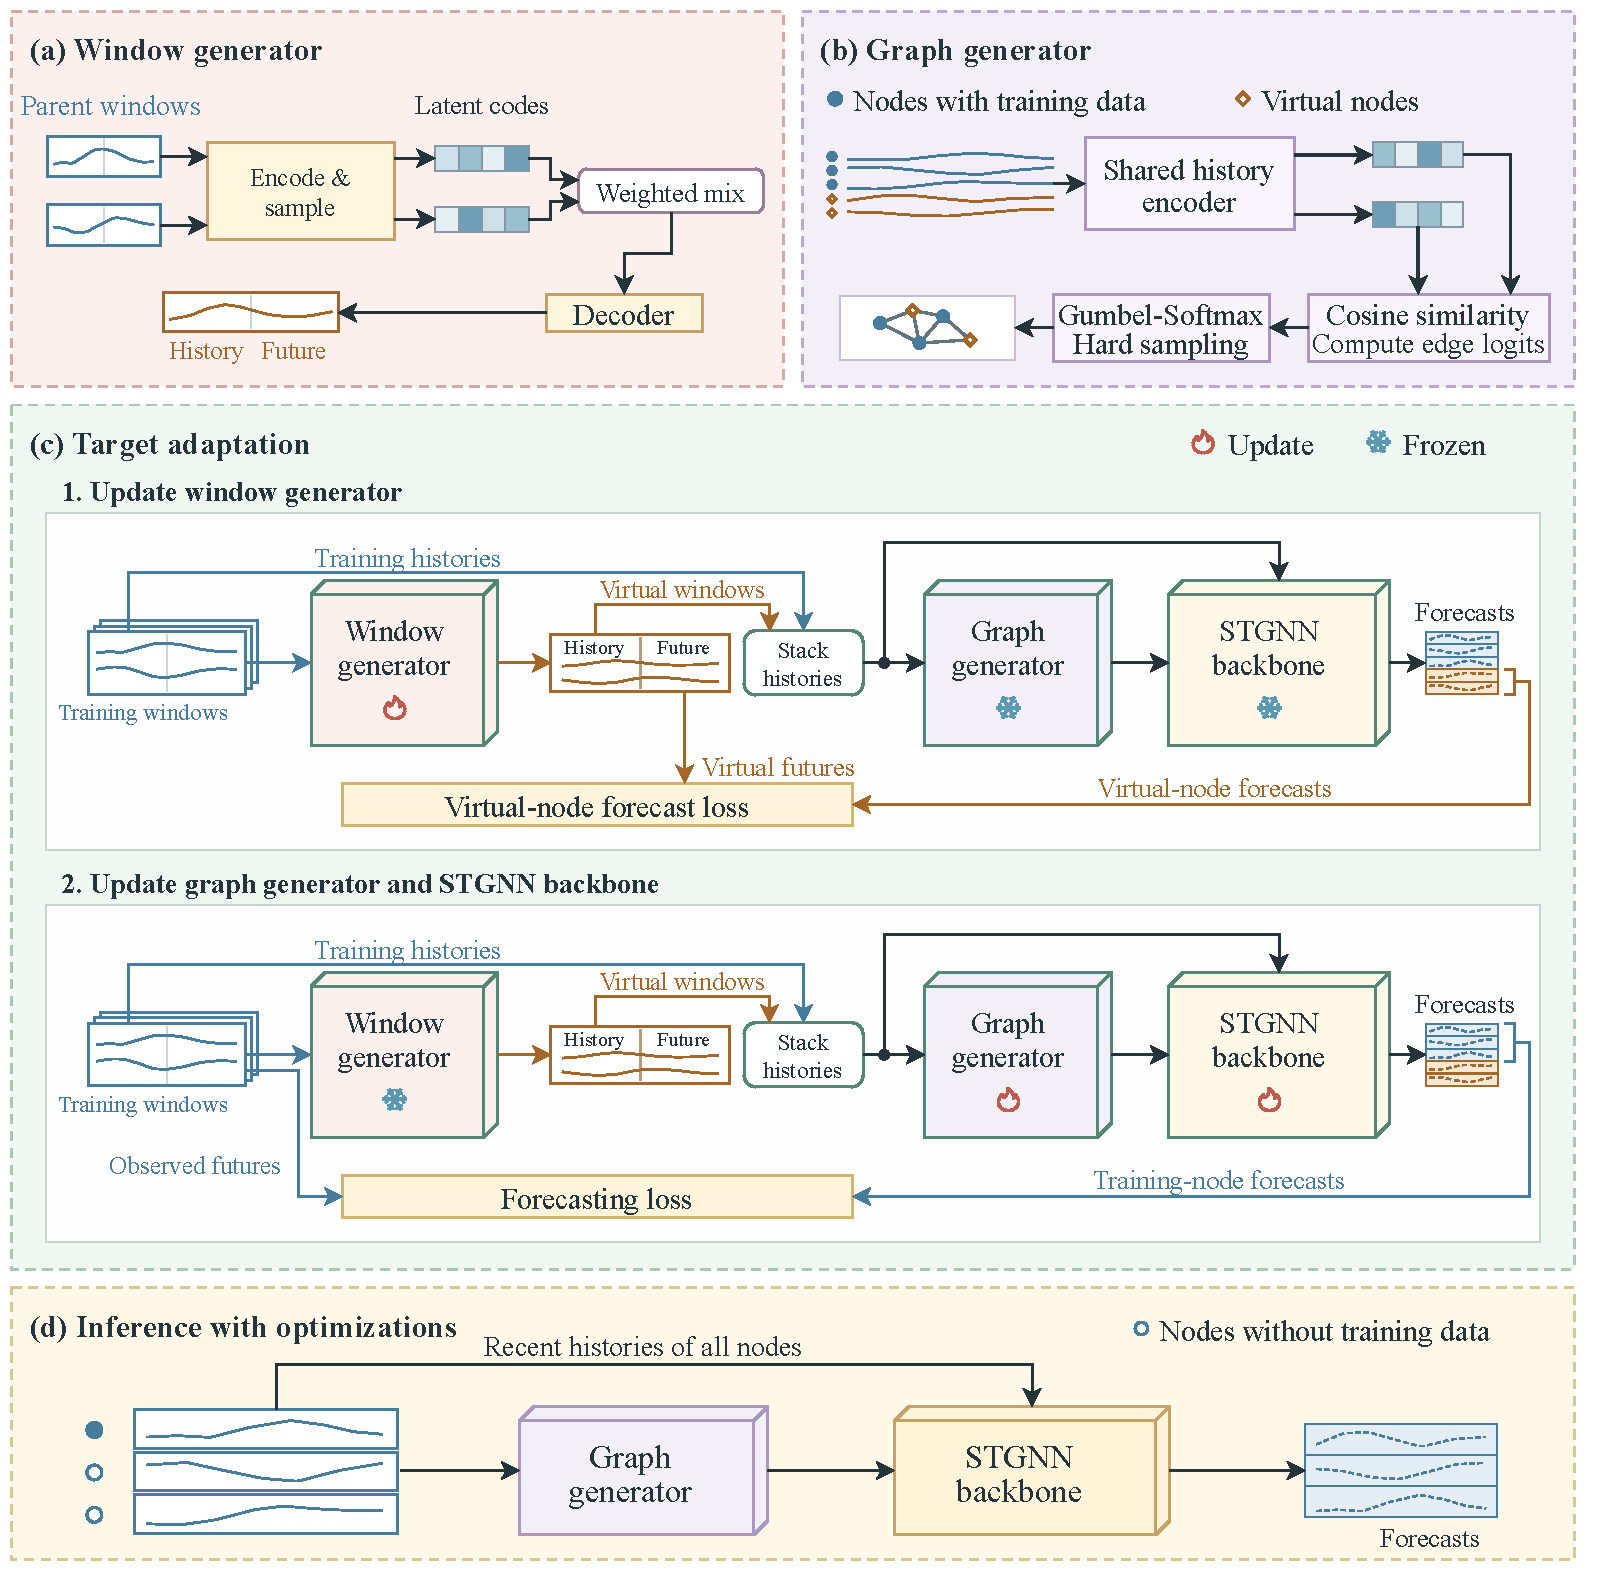
\includegraphics[width=0.92\textwidth]{images/method-overview.pdf}
\caption{Overview of CrossGEN. Panel (a) details the window generator. Panel (b) details the graph generator. Panel (c) shows target adaptation from source-pretrained weights for the transferred modules, including the alternating updates and their forecasting loss terms. Panel (d) shows inference with the window generator disabled.}
\label{fig:method-overview}
\end{figure}

\subsection{Window Generator}
\label{sec:node-generator}

\textbf{To address the first challenge of capturing temporal patterns beyond those observed at target training nodes}, CrossGEN transfers a window generator pretrained on source-city observations. Following ST-FiT's augmentation mechanism, the generator mixes the latent codes of two real traffic windows and decodes the resulting code into a virtual training window.

During target adaptation, the real windows come from nodes in $\mathcal O_T$. We standardize target traffic observations using $\mathcal S_T(x)=(x-m_T)/s_T$, where $m_T$ and $s_T>0$ are the mean and standard deviation computed from the training windows at the target training nodes; the window generator and STGNN backbone both output standardized values, with $\overline H_i^{(t)}$ and $\overline Y_i^{(t)}$ the standardized versions of $H_i^{(t)}$ and $Y_i^{(t)}$. A variational encoder~\cite{vae} maps each complete window $U_i^{(t)}=(\overline H_i^{(t)},\overline Y_i^{(t)})$ in $\mathbb R^{P+Q}$ to Gaussian distribution parameters, and a latent code is then sampled with an adjustable scale,
\begin{equation}
  (\mu_i^{(t)},\ell_i^{(t)})=E_\theta(U_i^{(t)}),\quad
  z_i^{(t)}=\mu_i^{(t)}+\rho\exp(\ell_i^{(t)}/2)\odot\epsilon_i^{(t)},\quad
  \epsilon_i^{(t)}\sim\mathcal N(0,I_d),
  \label{eq:latent-code}
\end{equation}
where the encoder $E_\theta$ and the decoder $D_\theta$ share parameters across nodes, $\rho$ scales the sampling standard deviation, and $\mu_i^{(t)}$, $\ell_i^{(t)}$ and $z_i^{(t)}$ are vectors in $\mathbb R^d$, with $d$ the latent dimension.

The codes of two parent windows are mixed with a ratio $\lambda$ as $\widetilde z_k^{(t)}=\lambda z_{i_k}^{(t)}+(1-\lambda)z_{j_k}^{(t)}$, and the decoder maps the mixed code back to a complete $P+Q$ window $\widetilde U_k^{(t)}=D_\theta(\widetilde z_k^{(t)})$, whose first $P$ steps form the history $\widetilde H_k^{(t)}\in\mathbb R^P$ and last $Q$ steps the future $\widetilde Y_k^{(t)}\in\mathbb R^Q$ (Fig.~\ref{fig:method-overview}(a)). We concatenate the virtual histories with the histories of the target training nodes for graph construction and forecasting (Fig.~\ref{fig:method-overview}(c)); in Phase 1, each virtual future supervises the corresponding virtual-node forecast. For convenience, we index the $K$ virtual nodes by $\mathcal K$ and use $\mathcal V^{+}=\mathcal O_T\cup\mathcal K$ to denote the node set used during adaptation, with $N_{\mathcal V^{+}}=N_{\mathrm{train}}+K$; the matrix $\overline H_{\mathcal V^{+}}^{(t)}\in\mathbb R^{N_{\mathcal V^{+}}\times P}$ has as its rows the standardized histories $\overline H_i^{(t)}$ of the target training nodes and the generated histories $\widetilde H_k^{(t)}$ of the virtual nodes.

To optimize the encoder and the decoder, we minimize the squared distance between a virtual window and its two parent windows together with the latent regularization term. To encourage temporal consistency across all $P+Q$ steps, we use the backbone on the sampled graph to forecast the future from the generated history. Let $\widehat{\overline Y}_{\mathcal V^{+}}^{(t)}\in\mathbb R^{N_{\mathcal V^{+}}\times Q}$ be the backbone output for the nodes in $\mathcal V^{+}$; for virtual node $k$, we compare the forecast $\widehat{\overline Y}_{k,q}^{(t)}$ with the generated value $\widetilde Y_{k,q}^{(t)}$ at each forecast step $q$, both in the standardized space. The window generator objective reads
\begin{equation}
\begin{aligned}
  \mathcal L_{\rm lat}^{(t)}&=\frac{1}{\text{$N_{\mathrm{train}}$}}\sum_{i\in\mathcal O_{T}}\sum_{r=1}^{d}
      \bigl((\mu_{i,r}^{(t)})^2+\exp(\ell_{i,r}^{(t)})-1-\ell_{i,r}^{(t)}\bigr),\\
  \mathcal L_{\rm par}^{(t)}&=\frac{1}{K(P+Q)}\sum_{k=1}^{K}
      \Bigl(\|\widetilde U_k^{(t)}-U_{i_k}^{(t)}\|_2^2+\|\widetilde U_k^{(t)}-U_{j_k}^{(t)}\|_2^2\Bigr),\\
  \mathcal L_{\rm vf}^{(t)}&=
      \text{$\displaystyle\frac{1}{KQ}\sum_{k\in\mathcal K}\sum_{q=1}^{Q}
      \left|\widehat{\overline Y}_{k,q}^{(t)}-\widetilde Y_{k,q}^{(t)}\right|$},
      \qquad\mathcal L_{\rm src}=\|\theta-\theta_S\|_2^2,\\
  \mathcal L_N^{(t)}&=\lambda_{\rm vf}\mathcal L_{\rm vf}^{(t)}+\lambda_{\rm lat}\mathcal L_{\rm lat}^{(t)}
      +\lambda_{\rm par}\mathcal L_{\rm par}^{(t)}+\lambda_{\rm src}\mathcal L_{\rm src},
\end{aligned}
  \label{eq:node-objectives}
\end{equation}
where the latent penalty acts on the unscaled means and log-variances, excluding the sampling scale $\rho$ in~\eqref{eq:latent-code}; the source penalty $\mathcal L_{\rm src}$ anchors $\theta$ to its source value; the parent-window penalty encourages a virtual window to retain the temporal patterns of both parents; and $\mathcal L_{\rm vf}^{(t)}$ encourages agreement between the backbone's forecast and the generated future.

\subsection{Graph Generator and STGNN Backbone}
\label{sec:graph-generator}

\textbf{To address the second challenge of inferring spatial dependencies without a predefined target adjacency matrix}, the graph generator builds connections between nodes from their temporal histories. During adaptation, it connects the target training nodes and the virtual nodes produced by the window generator (Fig.~\ref{fig:method-overview}(b)); at inference, the same construction uses the recent histories of all target nodes, including those without training data (Fig.~\ref{fig:method-overview}(d)).

A shared encoder first maps each history to a representation, and the cosine similarity between two representations gives an edge score,
\begin{equation}
  v_a^{(t)}=g_\phi(\overline H_a^{(t)}),\quad e_a^{(t)}=\frac{v_a^{(t)}}{\max(\|v_a^{(t)}\|_2,\epsilon_e)},\quad
  s_{ab}^{(t)}=\langle e_a^{(t)},e_b^{(t)}\rangle,\quad a,b\in\mathcal V^{+} ,
  \label{eq:graph-history-scores}
\end{equation}
where $a$ and $b$ range over $\mathcal V^{+}$ and $\overline H_a^{(t)}\in\mathbb R^{P}$ is the standardized history of node $a$, with $\overline H_a^{(t)}=\widetilde H_a^{(t)}$ when $a\in\mathcal K$. We use $\tilde A^{(t)}=G_\phi(\overline H_{\mathcal V^{+}}^{(t)})$ to denote the sampled adjacency. To sample each edge, we normalize the scores within the window, shift them by $\delta$, and exponentiate the shifted scores with scale $\alpha$ to obtain edge-present and edge-absent logits; a hard Gumbel-Softmax~\cite{gumbel} draw via $\operatorname{GS}^{\rm hard}_{\tau}$ at temperature $\tau$ then gives the edge,
\begin{equation}
\begin{aligned}
  r_{ab}^{(t)}&=\frac{s_{ab}^{(t)}-s_{\min}^{(t)}}{\max(s_{\max}^{(t)}-s_{\min}^{(t)},\epsilon_r)}-\delta,\\
  \ell_{ab}^{(t),\rm on}&=\exp(\alpha r_{ab}^{(t)}),\qquad
  \ell_{ab}^{(t),\rm off}=\exp(-\alpha r_{ab}^{(t)}),\\
  \tilde A_{ab}^{(t)}&=\left[\operatorname{GS}^{\rm hard}_{\tau}(\ell_{ab}^{(t),\rm on},\ell_{ab}^{(t),\rm off})\right]_{\rm on},
  \qquad \tau>0 ,
\end{aligned}
  \label{eq:sparse-graph}
\end{equation}
so that the graph is discrete while gradients still propagate through the sampled edges. Here $s_{\min}^{(t)}$ and $s_{\max}^{(t)}$ are the minimum and maximum scores within the window, $\epsilon_e$ and $\epsilon_r$ are numerical stability constants, and the resulting adjacency matrix $\tilde A^{(t)}$ has shape $N_{\mathcal V^{+}}\times N_{\mathcal V^{+}}$. The shared encoder and scoring function apply to node sets of different sizes, and higher scores favor edge inclusion. CrossGEN transfers the learned parameters of the graph generator and samples new edges from the histories available in the target city.

The STGNN backbone $F_\psi$ takes standardized node histories $\overline H^{(t)}$ and the adjacency matrix $\tilde A^{(t)}$ as input and outputs a $Q$-step forecast for each node; with the residual correction of Section~\ref{sec:target-adaptation}, it also receives the relation matrix $C^{(t)}$, so $\widehat{\overline Y}^{(t)}=F_\psi(\overline H^{(t)},\tilde A^{(t)},C^{(t)})$. During adaptation, the backbone receives $\overline H_{\mathcal V^{+}}^{(t)}$ (Fig.~\ref{fig:method-overview}(c)); at inference, it receives the standardized recent histories $\overline H_{\mathcal V_T}^{(t)}$ of all target nodes (Fig.~\ref{fig:method-overview}(d)). Its blocks follow the STGCN design~\cite{stgcn}, and $\psi$ is shared by all nodes, so the backbone applies to real and virtual nodes alike.

\subsection{Target Adaptation and Inference}
\label{sec:target-adaptation}
\label{sec:optimization-inference}

\textbf{To address the third challenge of source--target mismatch}, we use a \emph{target adaptation} pipeline designed to adapt the transferred modules while limiting their parameter deviation from the pretrained values. CrossGEN initializes the window generator, the graph generator and the backbone with source-pretrained weights. CrossGEN-W initializes only the window generator with source-pretrained weights and initializes the other two modules from scratch. NT initializes all three modules from scratch. These configurations therefore differ in which modules receive source initialization. All three construct target-side edges from the histories of the target training nodes and the virtual nodes (Fig.~\ref{fig:method-overview}(c)). Transfer requires matching $P$ and $Q$, and compatible parameter shapes, but no correspondence between the two node sets.

A target-initialized gated residual correction adjusts the backbone's graph-convolution messages to the target city. To limit parameter deviation, we regularize the source-loaded parameters toward their pretrained values and freeze them in the initial epochs. Specifically, the correction centers and normalizes the $i$-th row of $\overline H_{\mathcal V^{+}}^{(t)}$ into $u_i^{(t)}$ and scores each node pair by the averaged cosine similarity of $u_i^{(t)}$ and $W_\phi u_i^{(t)}$,
\begin{equation}
  b_{ij}^{(t)}=\left[\tfrac12\left((u_i^{(t)})^\top u_j^{(t)}+(W_\phi u_i^{(t)})^\top(W_\phi u_j^{(t)})\right)\right]_{[0,1]},
  \qquad b_{ii}^{(t)}=0 ,
  \label{eq:correction-scores}
\end{equation}
where $[\cdot]_{[0,1]}$ clips to the unit interval. Let $\Pi^{(t)}\in[0,1]^{N_{\mathcal V^{+}}\times N_{\mathrm{train}}}$ encode the parents for the window at $t$. We set $\Pi_{i,i}^{(t)}=1$ for $i\in\mathcal O_T$. For a virtual node $k$ with parents $i_k$ and $j_k$, we set $\Pi_{k,i_k}^{(t)}=\lambda$ and $\Pi_{k,j_k}^{(t)}=1-\lambda$. A sparse relation matrix $C^{(t)}\in\mathbb R^{N_{\mathcal V^{+}}\times N_{\mathcal V^{+}}}$ keeps at most the four largest entries of each row and normalizes each row by its retained sum; the rows of virtual nodes are then mixed by their parent weights $\Pi^{(t)}$. The gated residual messages are then added to the graph convolution,
\begin{equation}
\begin{aligned}
  Z^{(t,l)}&=\operatorname{TempConv}_1(H^{(t,l)}),\\
  H^{(t,l+1)}&=\operatorname{ChebConv}(Z^{(t,l)};\tilde A^{(t)})+\tanh(\gamma)\,R(C^{(t)}Z^{(t,l)}-Z^{(t,l)}),
\end{aligned}
  \label{eq:sparse-correction}
\end{equation}
where $H^{(t,l)}$ is the input of block $l$ for the window at $t$ (the superscript $(t,l)$ indexes the window time and the network block, respectively), $R$ a block-wise bias-free map and $\gamma$ the gate. For the $N_{\mathcal V^{+}}$ nodes in $\mathcal V^{+}$, $Z^{(t,l)}\in\mathbb R^{L_l\times N_{\mathcal V^{+}}\times d_l}$, where $L_l$ and $d_l$ are the number of time steps and feature channels after the first temporal convolution. At each time step, $C^{(t)}$ acts along the node axis of $Z^{(t,l)}$ and $R$ acts along the feature axis of the residual. The gate starts at zero, so the residual term initially vanishes. The correction parameters belong to $\psi$ but are excluded from source loading and source regularization. The STGNN backbone in Fig.~\ref{fig:method-overview}(c) and (d) includes this correction.

\paragraph{Alternating target adaptation.}
The modules depend on one another during adaptation. The window generator uses the backbone's forecasts to evaluate its virtual windows. The graph generator samples a graph from the concatenated real and virtual histories, and the STGNN backbone uses these histories and the sampled graph for forecasting. We train the modules by alternating between the two phases shown in Fig.~\ref{fig:method-overview}(c), using the window generator objective above and the forecasting objective below.

In Phase 1, we update the window generator with $\mathcal L_N^{(t)}$ and freeze the graph generator and STGNN backbone. The virtual-node forecast loss compares the predicted futures of virtual nodes with their generated futures. In Phase 2, we freeze the window generator and jointly update the graph generator and STGNN backbone. The forecasting loss compares training-node forecasts with observed futures. The regularization term anchors source-loaded parameters to their pretrained values,
\begin{equation}
\begin{aligned}
  C^{(t)}&=C_\phi(\overline H_{\mathcal V^{+}}^{(t)},\Pi^{(t)}),\qquad
  \widehat{\overline Y}_{\mathcal V^{+}}^{(t)}=F_\psi(\overline H_{\mathcal V^{+}}^{(t)},\tilde A^{(t)},C^{(t)}),\\
  \widehat Y_{\mathcal O_{T}}^{(t)}&=\mathcal S_T^{-1}([\widehat{\overline Y}_{\mathcal V^{+}}^{(t)}]_{\mathcal O_{T}}),\\
  \mathcal L_{\rm pred}^{(t)}&=\frac{1}{\text{$N_{\mathrm{train}}$}Q}\sum_{i\in\mathcal O_{T}}\sum_{q=1}^{Q}
      |\widehat Y_{i,q}^{(t)}-Y_{i,q}^{(t)}|,\\
  \mathcal L_{GF}^{(t)}&=\mathcal L_{\rm pred}^{(t)}
      +\lambda_{GF}\sum_{p\in\mathcal P_S}\|p-p_S\|_2^2,
\end{aligned}
  \label{eq:target-objectives}
\end{equation}
where $\mathcal P_S$ collects the source-loaded parameters of the two modules. The notation $[\cdot]_{\mathcal O_T}$ selects the rows for the target training nodes. The two loss boxes in Fig.~\ref{fig:method-overview}(c) show the forecasting terms $\mathcal L_{\rm vf}^{(t)}$ and $\mathcal L_{\rm pred}^{(t)}$, respectively. In this way, the window generator supplies virtual windows for forecasting, while the graph generator supplies the graph used by the backbone.

\paragraph{All-node inference.}
At inference (Fig.~\ref{fig:method-overview}(d)), we disable the window generator and standardize the recent histories of all target nodes as $\overline H_{\mathcal V_T}^{(t)}=\mathcal S_T(H_{\mathcal V_T}^{(t)})$. The adapted graph generator $G_{\phi^\star}$ builds the graph $\tilde A^{(t)}$ from these histories. The STGNN backbone $F_{\psi^\star}$ uses the same histories, the generated graph and the residual relations $C^{(t)}$ computed by $C_{\phi^\star}$ to forecast all target nodes. We apply $\mathcal S_T^{-1}$ to the standardized forecasts $\widehat{\overline Y}_{\mathcal V_T}^{(t)}$ to obtain $\widehat Y_{\mathcal V_T}^{(t)}$ before computing the evaluation metrics.


\subsection{Source Dataset Selection}
\label{sec:source-selection}

To prioritize candidate source datasets, we compute statistics from historical traffic observations at selected source nodes and target training nodes in the training splits. These statistics use no target test observations and require no correspondence between source and target nodes. We define a node distance $A(S,T)$ and a relationship distance $D(S,T)$ for a candidate source dataset $S$ and target dataset $T$.

The node distance $A(S,T)$ compares seven statistics per node, comprising the normalized mean absolute change between consecutive time steps and autocorrelations at six lags. The relationship distance $D(S,T)$ compares distributions of residual correlations between node pairs. We compute these correlations within each dataset after controlling for the predicted node's recent observations and daily and weekly cycles.

The scores are
\[
s_{\text{CrossGEN-W}}(S,T)=A(S,T),\qquad
s_{\text{CrossGEN}}(S,T)=0.25A(S,T)+0.75D(S,T).
\]
We rank candidate sources from lowest to highest score. The score weights were calibrated using earlier transfer results, so the source-ranking analysis in Section~\ref{sec:source} is retrospective. These scores provide a prioritization rule rather than a guarantee of positive transfer.

\section{Experiments}\label{sec:results}
\begin{samepage}
Our experiments address the following four research questions.
\begingroup
\DeclareRobustCommand{\revisedresearchquestions}{%
  \begin{itemize}
  \item \textbf{RQ1.} Compared with the baselines, how well does CrossGEN forecast traffic at target nodes, particularly those without training data?
  \item \textbf{RQ2.} How does the choice of which CrossGEN modules are initialized with source-pretrained weights affect forecasting on the target training data?
  \item \textbf{RQ3.} How does the choice of source dataset affect forecasting performance for a given target dataset?
  \item \textbf{RQ4.} How does target training-node coverage affect CrossGEN's forecasting performance?
  \end{itemize}%
}
\revisedresearchquestions
\endgroup
\end{samepage}

\subsection{Experimental Settings}
\label{sec:experimental-settings}


\noindent\textbf{Datasets.} We use seven datasets (Table~\ref{tab:datasets}), including five traffic flow datasets and two traffic index datasets.

\DeclareRobustCommand{\datasetvariablelist}{%
  \begin{itemize}
  \item \emph{Traffic flow datasets.} Traffic flow is the number of vehicles counted at a sensor in each interval. \textbf{PEMS03}, \textbf{PEMS04}, and \textbf{PEMS08} are existing benchmarks based on data from the Caltrans Performance Measurement System (PeMS)~\cite{pems}, with sensors in Districts 3, 4, and 8, respectively~\cite{stfit}. \textbf{CA03} and \textbf{CA06} are subsets that we construct from LargeST's California dataset~\cite{largest} by selecting sensors in Districts 3 and 6, respectively.
  \item \emph{Traffic index datasets.} The traffic index is a road-level measure of traffic congestion. \textbf{Shenzhen} and \textbf{Chengdu} are existing traffic index datasets with observations from roads in downtown Shenzhen and the core urban area of Chengdu, respectively. Both datasets come from the DiDi Chuxing GAIA Initiative~\cite{stgfsl} and are distributed through OpenCity~\cite{opencity}.
  \end{itemize}%
}
\datasetvariablelist

\begin{table}[!ht]
\centering
\DeclareRobustCommand{\datasetstatisticstable}{%
\caption{Dataset characteristics.}
\label{tab:datasets}
\footnotesize
\setlength{\tabcolsep}{1pt}
\renewcommand{\arraystretch}{1.1}
\begin{tabular*}{\linewidth}{@{\extracolsep{\fill}}lllrr@{}}
\hline
Dataset & Location & Variable & Nodes & Time steps \\
\hline
PEMS03 & Caltrans District 3, USA & Traffic flow & 358 & 26,208 \\
PEMS04 & Caltrans District 4, USA & Traffic flow & 307 & 16,992 \\
PEMS08 & Caltrans District 8, USA & Traffic flow & 170 & 17,856 \\
CA03 & Caltrans District 3, USA & Traffic flow & 441 & 25,920 \\
CA06 & Caltrans District 6, USA & Traffic flow & 456 & 25,920 \\
Shenzhen & Shenzhen, China & Traffic index & 627 & 17,280 \\
Chengdu & Chengdu, China & Traffic index & 524 & 17,280 \\
\hline
\end{tabular*}%
}
\datasetstatisticstable
\end{table}

\begingroup
\DeclareRobustCommand{\baselinecomparison}{%
  \noindent\textbf{Baselines.} We consider the following baselines.
  \begin{itemize}
  \item \textbf{Historical Average (HA)}~\cite{dai2020hstgcn} averages historical traffic observations.
  \item \textbf{FC-LSTM}~\cite{sutskever2014seq2seq} forecasts traffic with a fully connected LSTM.
  \item \textbf{STGCN}~\cite{stgcn} combines graph and temporal convolutions.
  \item \textbf{STGODE}~\cite{fang2021stgode} combines graph ordinary differential equations with temporal convolutions.
  \item \textbf{ST-FiT}~\cite{stfit} uses virtual nodes and a learned graph.
  \end{itemize}%
}
\begin{samepage}
\baselinecomparison
\end{samepage}
\endgroup

\begingroup
\DeclareRobustCommand{\evaluationmetrics}{%
\begin{samepage}
  \textbf{Evaluation Metric.} Let $\mathcal T_{\mathrm{test}}$ contain the time indices $t$ from which we make test forecasts, with $T_{\mathrm{test}}=|\mathcal T_{\mathrm{test}}|$. For a set $\mathcal A\subseteq\mathcal V_T$ of $N_{\mathcal A}$ target nodes, the mean absolute error (MAE) at forecast step $q$ is
\[
  \operatorname{MAE}_{q}(\mathcal A)
  = \frac{1}{T_{\mathrm{test}}N_{\mathcal A}}
    \sum_{t\in\mathcal T_{\mathrm{test}}}\sum_{i\in\mathcal A}
    \left|\widehat Y_{i,q}^{(t)}-Y_{i,q}^{(t)}\right|.
\]
We compute MAE on the original data scale and average it over all $Q$ forecast steps.
\end{samepage}
We report MAE for $\mathcal A\in\{\mathcal V_T,\mathcal O_T,\mathcal U_T\}$.
Where we train with five random seeds, we report MAE averaged over the five runs. We compare CrossGEN with the other methods using a two-sided paired $t$-test on MAE across all target nodes, matching runs by random seed. We use unadjusted $p$ values.
}
\noindent\evaluationmetrics
\endgroup

\noindent\textbf{Implementation Settings.}
The history and forecast lengths are both 12 time steps ($P=Q=12$). The forecast horizon is 1h for traffic flow at 5min intervals and 2h for traffic index at 10min intervals.

The main experiments use $N_{\mathrm{train}}=\lfloor 0.1 N_T\rfloor$ target training nodes.
For our runs, we use a chronological 6:2:2 split for training, validation, and testing.




Each main experiment uses a specified source dataset and target dataset. We train and evaluate CrossGEN with five random seeds and use the same seeds for ST-FiT on each target dataset.
We pretrain for 50 epochs on all source nodes with historical traffic observations.
We train for up to 100 epochs on the target data, with early stopping after 20 consecutive validation checks without improvement.
Training uses Adam (learning rate $2\times10^{-3}$, weight decay $10^{-4}$) with batch size 4.
The window generator uses $d=64$, $\lambda=0.5$, and $K=N_{\mathrm{train}}$. The graph generator uses $\delta=0.9$, $\alpha=10$, and $\tau=1$.





CrossGEN is pretrained on each listed source dataset and adapted using the same target training nodes and temporal split. All other methods use only target training data: ST-FiT is trained from scratch on this data, and the four reference methods are evaluated on the target test data. We report MAE on CA03, CA06, Shenzhen, and Chengdu, and use the reference values from Table~1 of Lei et al.~\cite{stfit} on PEMS03, PEMS04, and PEMS08. All methods are evaluated on the same target test data and all target nodes.

\subsection{Overall Results (RQ1)}
\label{sec:overall-results}









Table~\ref{tab:main-results} reports the results across all target nodes for the traffic flow and traffic index experiments. Methods that use only target training data each have one result per target dataset, and CrossGEN, the only cross-city method in the table, has one result per line.

CrossGEN achieves lower MAE than all other methods for all traffic index experiments and for all traffic flow experiments except the experiment from CA06 to PEMS08. On PEMS08, ST-FiT achieves the lowest MAE when CA06 is the source, whereas CrossGEN achieves lower MAE than ST-FiT with PEMS03 or PEMS04 as the source. Source pretraining can help the window generator capture temporal patterns that are underrepresented in the target training data and help the graph generator identify informative neighbors from target histories. These benefits depend on how well the learned temporal patterns and spatial dependencies carry over to the target. The CA06 to PEMS08 result is consistent with a mismatch in spatial dependencies. When the transferred graph generator and STGNN backbone favor spatial dependencies that differ from those in the target, regularization toward the source weights can make it harder to adjust edge scores and neighbor aggregation using data from only a subset of target nodes.

\begin{table}[t]
\centering
\caption{Forecasting results across all target nodes.}
\label{tab:main-results}
\footnotesize
\setlength{\tabcolsep}{2.2pt}
\begin{tabular}{@{}llrrrr@{\hspace{9pt}}rr@{}}
\hline

\shortstack[l]{Target\\dataset} & \shortstack[l]{Source\\dataset} &
HA & FC-LSTM & STGCN & STGODE & ST-FiT & CrossGEN \\
\hline
\multirow{3}{*}{PEMS03} & CA06 &
  \multirow{3}{*}{32.47} & \multirow{3}{*}{20.56} &
  \multirow{3}{*}{23.22} & \multirow{3}{*}{31.05} &
  \multirow{3}{*}{18.86} & \textbf{18.35} \\
 & PEMS04 & & & & & & \textbf{18.03} \\
 & PEMS08 & & & & & & \textbf{18.43} \\[3pt]
\multirow{3}{*}{PEMS04} & CA06 &
  \multirow{3}{*}{41.98} & \multirow{3}{*}{28.17} &
  \multirow{3}{*}{32.60} & \multirow{3}{*}{34.35} &
  \multirow{3}{*}{25.23} & \textbf{24.57} \\
 & PEMS03 & & & & & & \textbf{24.83} \\
 & PEMS08 & & & & & & \textbf{24.55} \\[3pt]
\multirow{3}{*}{PEMS08} & CA06 &
  \multirow{3}{*}{34.56} & \multirow{3}{*}{30.52} &
  \multirow{3}{*}{41.67} & \multirow{3}{*}{30.00} &
  \multirow{3}{*}{23.15} & 23.55 \\
 & PEMS03 & & & & & & \textbf{23.00} \\
 & PEMS04 & & & & & & 23.05 \\[3pt]
\multirow{2}{*}{CA03} & CA06 &
  \multirow{2}{*}{36.65} & \multirow{2}{*}{26.43} &
  \multirow{2}{*}{32.64} & \multirow{2}{*}{30.98} &
  \multirow{2}{*}{21.35} & \textbf{21.15} \\
 & PEMS04 & & & & & & \textbf{21.34} \\[3pt]
\multirow{3}{*}{CA06} & CA03 &
  \multirow{3}{*}{30.28} & \multirow{3}{*}{28.23} &
  \multirow{3}{*}{21.74} & \multirow{3}{*}{24.74} &
  \multirow{3}{*}{16.74} & \textbf{16.07} \\
 & PEMS03 & & & & & & \textbf{16.36} \\
 & PEMS04 & & & & & & \textbf{16.49} \\
\hline
Shenzhen & Chengdu & 4.27 & 3.68 & 3.17 & 3.37 & 2.90 & \textbf{2.77} \\
Chengdu & Shenzhen & 5.02 & 4.40 & 3.63 & 4.14 & 3.12 & \textbf{3.07} \\
\hline
\end{tabular}\par
\end{table}

\subsection{Ablation Study (RQ2)}
\label{sec:configuration-scope}

\begingroup
\DeclareRobustCommand{\ablationpar}{\par}



\DeclareRobustCommand{\ablationvariants}{%
  \begin{samepage}
    Each model variant trains all three modules on the target training data.
    \begin{enumerate}
    \item \textbf{NT (no transfer)} initializes each module from scratch.
    \item \textbf{CrossGEN-W} (W for window) initializes only the window generator with source-pretrained weights and initializes the graph generator and STGNN backbone from scratch.
    \item \textbf{CrossGEN} initializes the window generator, graph generator, and STGNN backbone with source-pretrained weights.
    \end{enumerate}
  \end{samepage}%
}
\ablationvariants
CrossGEN-W helps assess transfer in two stages. Comparing NT with CrossGEN-W measures the effect of initializing the window generator with source-pretrained weights. Comparing CrossGEN-W with CrossGEN evaluates the joint effect of transferring the graph generator and STGNN backbone and applying the corresponding target-adaptation design.
\ablationpar
Table~\ref{tab:group-results} reports the results separately for target nodes with and without training data.
Compared with NT, CrossGEN-W and CrossGEN achieve lower MAE across all target nodes in 10 and 11 of the 14 traffic flow experiments and in both traffic index experiments, respectively. The comparison confirms the effectiveness of the transfer: initializing the window generator with source-pretrained weights improves forecasting, and additionally transferring the graph generator and the backbone brings further gains. On PEMS08, however, CrossGEN-W outperforms CrossGEN in all experiments.
\par
\endgroup

\begin{table}[!htbp]
\centering
\caption{Ablation results by target node group.}
\label{tab:group-results}
\footnotesize
\setlength{\tabcolsep}{3pt}
\begin{tabular}{@{}llrr|rr|rr@{}}
\hline
\multirow{2}{*}{\shortstack[l]{Target\\dataset}} &
\multirow{2}{*}{\shortstack[l]{Source\\dataset}} &
\multicolumn{2}{c|}{NT} & \multicolumn{2}{c|}{CrossGEN-W} & \multicolumn{2}{c}{CrossGEN} \\
 & & $\mathcal O_{T}$ & $\mathcal U_T$ & $\mathcal O_{T}$ & $\mathcal U_T$ & $\mathcal O_{T}$ & $\mathcal U_T$ \\
\hline
PEMS03 & CA06 & 18.35 & 18.92 & \textbf{18.06} & 18.37 & 18.21 & \textbf{18.37} \\
PEMS03 & PEMS04 & 18.35 & 18.92 & 18.42 & 18.34 & \textbf{17.90} & \textbf{18.04} \\
PEMS03 & PEMS08 & 18.35 & 18.92 & 18.97 & 18.59 & \textbf{17.71} & \textbf{18.51} \\
PEMS04 & CA06 & 23.80 & 25.39 & 24.17 & 25.82 & \textbf{23.26} & \textbf{24.71} \\
PEMS04 & PEMS03 & 23.80 & 25.39 & \textbf{22.59} & 25.28 & 23.60 & \textbf{24.96} \\
PEMS04 & PEMS08 & 23.80 & 25.39 & \textbf{23.24} & 25.31 & 23.92 & \textbf{24.62} \\
PEMS08 & CA06 & 24.79 & 22.97 & \textbf{23.98} & \textbf{22.21} & 25.11 & 23.38 \\
PEMS08 & PEMS03 & 24.79 & 22.97 & \textbf{23.13} & \textbf{22.03} & 24.71 & 22.81 \\
PEMS08 & PEMS04 & 24.79 & 22.97 & \textbf{23.01} & \textbf{21.36} & 24.47 & 22.89 \\
CA03 & CA06 & 19.25 & 21.58 & 19.49 & 21.64 & \textbf{18.99} & \textbf{21.39} \\
CA03 & PEMS04 & 19.25 & \textbf{21.58} & 19.72 & 21.95 & \textbf{18.45} & 21.66 \\
CA06 & CA03 & 18.29 & 16.57 & 17.65 & 16.28 & \textbf{17.31} & \textbf{15.93} \\
CA06 & PEMS03 & 18.29 & 16.57 & \textbf{17.31} & 16.23 & 18.42 & \textbf{16.13} \\
CA06 & PEMS04 & 18.29 & 16.57 & 17.61 & \textbf{16.30} & \textbf{17.46} & 16.39 \\
\hline
Shenzhen & Chengdu & 2.82 & 2.91 & 2.68 & 2.83 & \textbf{2.68} & \textbf{2.78} \\
Chengdu & Shenzhen & 2.83 & 3.16 & 2.87 & 3.16 & \textbf{2.76} & \textbf{3.10} \\
\hline
\end{tabular}\par
\end{table}

\subsection{Source Dataset Selection (RQ3)}
\label{sec:source}
The temporal patterns and spatial dependencies learned during source pretraining depend on the source dataset, so the choice of the source dataset can affect the target MAE. Figure~\ref{fig:source-ranking-bars} ranks the candidate sources by MAE for each traffic flow target under CrossGEN. Each traffic index target has only one candidate source, so the analysis focuses on the traffic flow targets.

\begin{figure}[!htbp]
\centering
\begin{subfigure}[t]{0.49\linewidth}
\centering
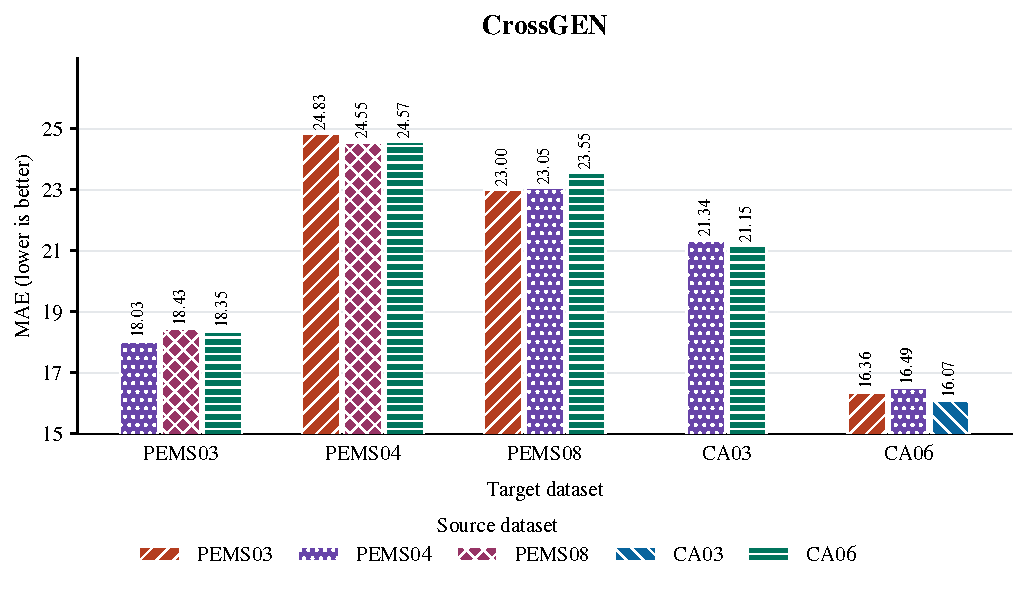
\includegraphics[width=\linewidth]{image/source-ranking-bars-crossgen.pdf}
\caption{Source dataset rankings for CrossGEN. Each group of bars shows the MAE of the candidate sources for a traffic flow target; lower is better.}
\label{fig:source-ranking-bars}
\end{subfigure}\hfill
\begin{subfigure}[t]{0.49\linewidth}
\centering
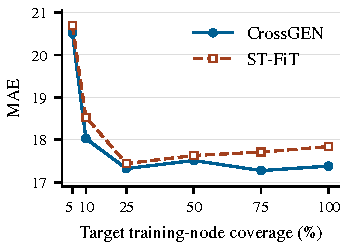
\includegraphics[width=\linewidth]{image/training-node-coverage.pdf}
\caption{MAE on PEMS03 by target training-node coverage. ST-FiT values were read from Fig.~3(a) of Lei et al.~\cite{stfit}.}
\label{fig:training-node-coverage}
\end{subfigure}
\caption{Source dataset selection and target training-node coverage.}
\end{figure}

The preferred source varies across targets. For example, on PEMS03 the lowest MAE comes from PEMS04, while on PEMS08 it comes from PEMS03, showing that the best source depends on the target dataset.

To examine whether more similar datasets yield lower MAE, we compare these observed rankings with the ranking produced by the dissimilarity score defined in Section~\ref{sec:source-selection}.

For each target dataset, we compare the candidate sources two at a time. The lower-scoring source has lower MAE in 9 of 13 comparisons, and the lowest-scoring source achieves the lowest MAE in 4 of the 5 traffic flow targets. On PEMS08, PEMS03 ranks first by both measures, while the score places CA06 ahead of PEMS04 even though PEMS04 has the lower MAE.

The agreement between the scores and MAE follows from what the two distances measure. The node distance $A(S,T)$ measures how similar the temporal patterns of the two cities are, indicating how much the source-pretrained window generator can contribute to the target. The relationship distance $D(S,T)$ measures how similar their spatial dependencies are, indicating how well the transferred graph generator and backbone can adapt. CrossGEN transfers both types of modules, and its score combines the two distances with a larger weight (0.75) on the relationship distance. The retrospective agreement suggests that these statistics can help shortlist sources for a given target, although using them as a selection rule would require validation on experiments outside the score calibration.

\subsection[Effect of Target Training-Node Coverage]{Effect of Target Training-Node Coverage (RQ4)}
\label{sec:training-node-coverage}



The main experiments use approximately 10\% target training-node coverage. To examine how sensitive forecasting is to the amount of target training data, we vary the fraction of PEMS03 nodes that supply historical traffic observations for training. Figure~\ref{fig:training-node-coverage} shows CrossGEN's MAE at the evaluated coverage levels alongside the published ST-FiT curve. All target nodes still provide recent observations at inference.

Both curves show their largest MAE reduction between the lowest coverage levels. MAE decreases further at intermediate coverage and fluctuates within a narrower range at higher coverage.

At low coverage, adding training nodes provides histories and forecast targets from more locations. This can help CrossGEN adapt the window generator to target temporal patterns and train the graph generator and STGNN backbone on a broader range of target observations. At higher coverage, additional nodes may contribute less information about patterns already represented in the training data.

On PEMS03, the coverage used in the main experiments lies in the range where MAE is most sensitive to how many nodes provide training data.

\section{ Conclusion}\label{sec:discussion}

In this paper, we propose CrossGEN for cross-city traffic forecasting with limited target training-node coverage.
CrossGEN transfers the pretrained weights of the window generator, graph generator, and STGNN backbone from a source city and adapts these modules using target training data.
Our experiments show that when few target nodes provide training data, cross-city transfer can improve forecasts at the remaining nodes.



\label{sec:conclusion}

% Anonymous submission: acknowledgments commented out; restore for the camera-ready version.
% \begin{credits}
% \subsubsection{\ackname}
% OpenAI Codex assisted with manuscript organization, drafting, revision, translation and literature summaries based on author-provided methods, derivations and records; experimental-table preparation (Section~\ref{sec:results}); ranking/error checks (Section~\ref{sec:source}); and design, drawing and export of the editable method figure (Fig.~\ref{fig:method-overview}).
%
% \end{credits}

% LNCS reference style; keys and bibliographic metadata retained.
\begin{thebibliography}{30}
\bibitem{boukerche2020traffic} Boukerche, A., Wang, J.: Machine Learning-based traffic prediction models for Intelligent Transportation Systems. Comput. Netw. \textbf{181}, 107530 (2020).
\bibitem{yin2022traffic} Yin, X., Wu, G., Wei, J., Shen, Y., Qi, H., Yin, B.: Deep Learning on Traffic Prediction: Methods, Analysis, and Future Directions. IEEE Trans. Intell. Transp. Syst. \textbf{23}(6), 4927--4943 (2022).
\bibitem{yuan2021traffic} Yuan, H., Li, G.: A Survey of Traffic Prediction: from Spatio-Temporal Data to Intelligent Transportation. Data Sci. Eng. \textbf{6}(1), 63--85 (2021). % https://doi.org/10.1007/s41019-020-00151-z
\bibitem{stfit} Lei, Z., Dong, Y., Li, J., Chen, C.: ST-FiT: Inductive Spatial-Temporal Forecasting with Limited Training Data. In: Proc. AAAI, pp. 12031--12039 (2025).
\bibitem{stgfsl} Lu, B., Gan, X., Zhang, W., Yao, H., Fu, L., Wang, X.: Spatio-Temporal Graph Few-Shot Learning with Cross-City Knowledge Transfer. In: Proc. ACM SIGKDD, pp. 1162--1172 (2022). 
\bibitem{transgtr} Jin, Y., Chen, K., Yang, Q.: Transferable Graph Structure Learning for Graph-Based Traffic Forecasting Across Cities. In: Proc. ACM SIGKDD, pp. 1032--1043 (2023).
\bibitem{stsurvey} Jin, G., Liang, Y., Fang, Y., Shao, Z., Huang, J., Zhang, J., Zheng, Y.: Spatio-Temporal Graph Neural Networks for Predictive Learning in Urban Computing: A Survey. IEEE Trans. Knowl. Data Eng. \textbf{36}(10), 5388--5408 (2024). 
\bibitem{stgcn} Yu, B., Yin, H., Zhu, Z.: Spatio-Temporal Graph Convolutional Networks: A Deep Learning Framework for Traffic Forecasting. In: Proc. IJCAI, pp. 3634--3640 (2018). 
\bibitem{dcrnn} Li, Y., Yu, R., Shahabi, C., Liu, Y.: Diffusion Convolutional Recurrent Neural Network: Data-Driven Traffic Forecasting. In: Proc. ICLR (2018).
\bibitem{graphwavenet} Wu, Z., Pan, S., Long, G., Jiang, J., Zhang, C.: Graph WaveNet for Deep Spatial-Temporal Graph Modeling. In: Proc. IJCAI, pp. 1907--1913 (2019). 
\bibitem{agcrn} Bai, L., Yao, L., Li, C., Wang, X., Wang, C.: Adaptive Graph Convolutional Recurrent Network for Traffic Forecasting. In: Advances in Neural Information Processing Systems, vol. 33, pp. 17804--17815 (2020).
\bibitem{mtgnn} Wu, Z., Pan, S., Long, G., Jiang, J., Chang, X., Zhang, C.: Connecting the Dots: Multivariate Time Series Forecasting with Graph Neural Networks. In: Proc. ACM SIGKDD, pp. 753--763 (2020). 
\bibitem{ignnk} Wu, Y., Zhuang, D., Labbe, A., Sun, L.: Inductive Graph Neural Networks for Spatiotemporal Kriging. In: Proc. AAAI, pp. 4478--4485 (2021). 
\bibitem{increase} Zheng, C., Fan, X., Wang, C., Qi, J., Chen, C., Chen, L.: INCREASE: Inductive Graph Representation Learning for Spatio-Temporal Kriging. In: Proc. ACM Web Conf., pp. 673--683 (2023). 
\bibitem{frigate} Gupta, M., Kodamana, H., Ranu, S.: Frigate: Frugal Spatio-temporal Forecasting on Road Networks. In: Proc. ACM SIGKDD, pp. 649--660 (2023). 
\bibitem{vae} Kingma, D.P., Welling, M.: Auto-Encoding Variational Bayes. In: Proc. ICLR (2014).
\bibitem{metast} Yao, H., Liu, Y., Wei, Y., Tang, X., Li, Z.: Learning from Multiple Cities: A Meta-Learning Approach for Spatial-Temporal Prediction. In: Proc. World Wide Web Conf., pp. 2181--2191 (2019). 
\bibitem{mtpb} Liu, Z., Zheng, G., Yu, Y.: Multi-scale Traffic Pattern Bank for Cross-city Few-shot Traffic Forecasting. ACM Trans. Knowl. Discov. Data \textbf{19}(4), Art. no. 94 (2025). 
\bibitem{stan} Fang, Z., Wu, D., Pan, L., Chen, L., Gao, Y.: When Transfer Learning Meets Cross-City Urban Flow Prediction: Spatio-Temporal Adaptation Matters. In: Proc. IJCAI, pp. 2030--2036 (2022). 
\bibitem{sert} Liu, Z., Sun, Z., Zhang, J., Zhang, B., Tong, P.: Regional Knowledge Transfer for Urban Traffic Flow Prediction via Satellite Imagery Assisted Contrastive Domain Adaptation. IEEE Trans. Intell. Transp. Syst. \textbf{26}(11), 19120--19134 (2025). 
\bibitem{traffictl} Huang, Y., Song, X., Zhu, Y., Zhang, S., Yu, J.J.Q.: Traffic Prediction With Transfer Learning: A Mutual Information-Based Approach. IEEE Trans. Intell. Transp. Syst. \textbf{24}(8), 8236--8252 (2023). 
\bibitem{crosscity} Deng, Z., Wu, Z., Su, L., Zhang, X., Wang, Y., Huang, Q.: Cross-City Correlation Learning for Traffic Forecasting. IEEE Trans. Intell. Transp. Syst. \textbf{27}(2), 2252--2267 (2026). 
\bibitem{gumbel} Jang, E., Gu, S., Poole, B.: Categorical Reparameterization with Gumbel-Softmax. In: Proc. ICLR (2017).
\bibitem{pems} California Department of Transportation: Caltrans Performance Measurement System (PeMS). https://pems.dot.ca.gov/, last accessed 2026/11/16.
\bibitem{largest} Liu, X., Xia, Y., Liang, Y., Hu, J., Wang, Y., Bai, L., Huang, C., Liu, Z., Hooi, B., Zimmermann, R.: LargeST: A Benchmark Dataset for Large-Scale Traffic Forecasting. In: Advances in Neural Information Processing Systems 36 (NeurIPS 2023).
\bibitem{opencity} Li, Z., Xia, L., Shi, L., Xu, Y., Yin, D., Huang, C.: Open Spatio-Temporal Foundation Models for Traffic Prediction. ACM Trans. Intell. Syst. Technol. (2025). 
\bibitem{dai2020hstgcn} Dai, R., Xu, S., Gu, Q., Ji, C., Liu, K.: Hybrid Spatio-Temporal Graph Convolutional Network: Improving Traffic Prediction with Navigation Data. In: Proc. ACM SIGKDD, pp. 3074--3082 (2020).
\bibitem{sutskever2014seq2seq} Sutskever, I., Vinyals, O., Le, Q.V.: Sequence to Sequence Learning with Neural Networks. In: Advances in Neural Information Processing Systems, vol. 27 (2014).
\bibitem{fang2021stgode} Fang, Z., Long, Q., Song, G., Xie, K.: Spatial-Temporal Graph ODE Networks for Traffic Flow Forecasting. In: Proc. ACM SIGKDD, pp. 364--373 (2021).
\bibitem{tldcrnn} Mallick, T., Balaprakash, P., Rask, E., Macfarlane, J.: Transfer Learning with Graph Neural Networks for Short-Term Highway Traffic Forecasting. In: Proc. ICPR, pp. 10367--10374 (2021).
\end{thebibliography}
\end{document}
